\section {Monotonicity of DFA Framework}
\setlength{\parindent}{0pt}
(Prepared by Sanket Gandhi)

\vspace{0.3cm}
\begin{itemize}
    \item Recall that we require semilatiice ($V$,\^{}) to have finite height with some properties over $F$ to guarantee convergence property of the fixed point  iteration.
    \item Also recall that family of transfer function have three properties, all functions in $F$ should be of form $V$ to $V$, $F$ should contain identity function and $F$ should be closed under composition. Do we have additional requirements from $F$ to guarantee convergence of fixed point iteration?
\end{itemize}

\subsection{Example}
Consider DFA ($F$,$V$,\^{})* with $V = \{true, false\}$, \^{}$= logical \ and $, $F = \{id,not,True,False\}$. The transfer functions are defined as follows:
\[id(x) = x, \ \ \forall x \in V \]
\[not(true) = false\]
\[not(false) = true\]
\[True(x) = true, \ \ \forall x \in V \]
\[False(x) = true, \ \ \forall x \in V \]
\begin{figure}[h!]
\caption{Semilattice diagram of *}
\begin{center}
\begin{tikzpicture}[-latex ,auto ,node distance =1.5cm and 2cm ,on grid ,
    semithick ,
    state/.style ={ rectangle ,top color =white , bottom color = blue!20 ,
    draw, blue , text=blue , scale = 0.7 ,minimum width =2.5 cm, minimum height = 1.1 cm}]
    \node[state] (A){} node [label = {}, rectangle split,rectangle split parts=2]{%
      true%
      };
    \node[state] (E) [below =of A]{} node [label = {},rectangle split,rectangle split parts=2] [below = of A] {%
      false%
      };
    \path[->] (A) edge node [above = 0.2 cm] {} (E);
    
\end{tikzpicture}
\end{center}
\label{fig:semilattice_and}
\end{figure}
\begin{itemize}
    \item Note that semilattice have finite height 2.
    \item Every function in $F$ is of form $V \rightarrow V$
    \item $F$ contains the identity function which is $id$.
    \item $F$ is closed under composition
\end{itemize}
The $F$ is valid family of transfer functions. Consider following instance of program. Basic block $B1$ have transfer function $id$ and basic block $B2$ have $not$ transfer function. By boundary condition and initialization of intermediate program point with top value the initial state is also shown in following figure. 
\begin{figure}[ht]
    \centering
    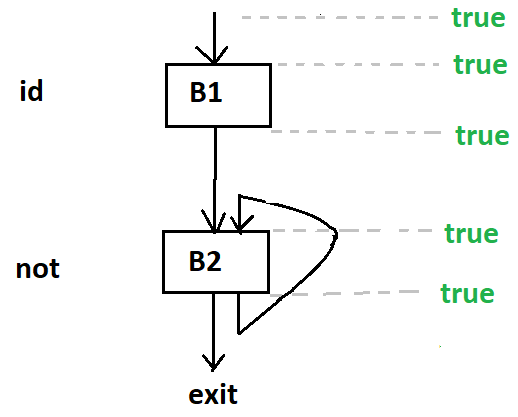
\includegraphics[scale= 0.4]{images/100-1.png}
    \caption{Initial State}
\end{figure}
When iterative fixed point algorithm first time reaches basic block $B2$ it meets over incoming  edges which is logical and of $true$. The out value of $B2$ and hence one of the in edge value of $B2$ become $not(true)$ which is $false$. The meet operator is logical and so the in value of $B2$ also becomes false.
\begin{figure}
    \centering
    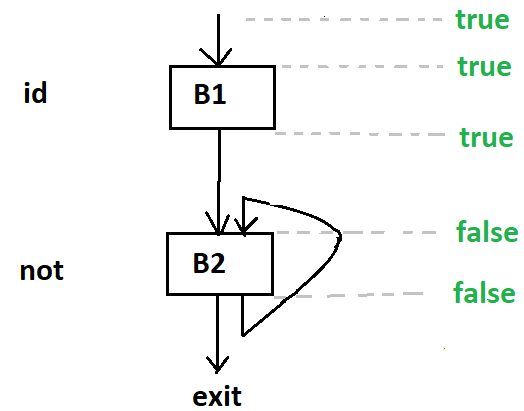
\includegraphics[scale= 0.4]{images/100-2.png}
    \caption{After FPI reaches B2 first time}
\end{figure}
As the $in[B2]$ and $out[B2]$ are not satisfying the transfer function condition FPI will again reach to $B2$. The $in[B2]$ and $out[B2]$ will again become $true$. Even our DFA framework follows all properties discussed earlier the algorithm will never converge. 
\begin{itemize}
    \item There should be some more constraints on family of transfer function $F$ so to guarantee convergence of FPI.  
    \item The problem is $not$ function in $F$ which keeps oscillating between two values. It is expected that the transfer function should keep same order in output values as that of input values(if it is defined).  
\end{itemize}
\subsection{Monotonicity of DFA framework}
A DFA framework ($F$,$V$,\^{}) is monotone if and only if
\[if \ \ \ \ x \leq y \ \ \ implies \ \ \ f(x) \leq f(y) \ \ \ \forall f \in F \ \ \ \ \forall x,y \in V\]
\begin{itemize}
    \item This says that if DFA framework is monotone then for all transfer functions in $F$ if there is particular order in input values then corresponding output values will also follow same order.
    \item In above examples $true \geq false$ but $not(true) \ngeq not(false)$, hence above DFA framework was not monotone.
    \item Equivalently a framework is monotone if and only if $f(x$\^{}$y) \leq f(x)$\^{}$f(y)$.
    The proof for DFA monotonicity implies $f(x$\^{}$y) \leq f(x)$\^{}$f(y)$ was provided in live session and is as follows:\\
    \textit{Proof:} By definition of meet operator,
    $a$\^{}$b \leq a$ and  $a$\^{}$b \leq b$. As DFA framework is monotone for all tansfer functions $f(a$\^{}$b) \leq f(a)$ and $f(a$\^{}$b) \leq f(b)$ holds. Now $f(a$\^{}$b) \leq f(b)$ implies $f(a$\^{}$b)$\^{}$f(b) = f(a$\^{}$b)$. Similarly $f(a$\^{}$b) \leq f(a)$ implies $f(a$\^{}$b)$\^{}$f(a) = f(a$\^{}$b)$. Now consider $(f(a)$\^{}$f(b))$\^{}$f(a$\^{}$b)$ is same as as $(f(a)$\^{}$f(b))$\^{}$(f(a$\^{}$b)$\^{}$f(a$\^{}$b))$. By using properties of meet operator the above expression is same as 
    $(f(a)$\^{}$f(a$\^{}$b))$\^{}$(f(b)$\^{}$f(a$\^{}$b))$. Which further boils down to $f(a$\^{}$b)$\^{}$f(a$\^{}$b)$ = $f(a$\^{}$b)$. At the end $(f(a)$\^{}$f(b))$\^{}$f(a$\^{}$b)$ = $f(a$\^{}$b)$. Therefore $f(a)$\^{}$f(b) \geq f(a$\^{}$b)$.
    \item Also in example discussed above $not(false$\^{}$true) = true$ and $not(true)$\^{}$not(false)=false$. Which means $not(false$\^{}$true) \nleq not(false)$\^{}$not(true)$ and so DFA framework in example was not monotone.

\subsection{Monotone DFA Example}
Consider the reaching definitions DFA ($F$,$V$,\^{}). The transfer function in this framework is of type $f(x) = (x-kill)\bigcup gen$. The values in this framework are set of definitions. If $x\leq y$ then this implies $x \supseteq y$ for $x,y \in V$. For transfer function $f\in F$ and $x_{1},x_{2} \in V$,
\[f(x_{1}) = (x_{1}-kill)\bigcup gen\]
\[f(x_{2}) = (x_{2}-kill)\bigcup gen\]
Clearly if $x_{1} \leq x_{2}$ implies $x_{1} \supseteq x_{2}$ which implies $f(x_{1}) \supseteq f(x_{2})$. This implies $f(x_{1}) \leq f(x_{2})$. This shows ($F$,$V$,\^{}) is monotone. 
\end{itemize}